%!TEX root=../main.tex
\section{Dataset} % (fold)
\label{sec:dataset}


We consider data from the National Basketball Association (NBA). To access comprehensive game data, we utilize the Python package \texttt{nba\_api}\footnote{\url{https://github.com/swar/nba_api/}}, which provides access to the APIs of \url{nba.com}. The dataset consists of both made and missed field goal attempt locations from the offensive half-court from all NBA games spanning the seasons between $2018-2019$ and $2022-2024$. Filtering the dataset, we focus solely on players who have made more than $1000$ field goal attempts during this six-season period, resulting in a cohort of $173$ players. These players accounted for a total of $717381$ shots attempted, of which $340466$ ($47\%$) were successful. Subsequently, we exclude shots deemed impossible (e.g., out-of-bounds), leaving us with a dataset comprising $715734$ shots, of which $340391$ ($47\%$) were successful.

Players are usually assigned to positions using their role on the court. The NBA caracterized players in three main positions: guard, forward and center. The guard is usually responsible to the handling of the ball, the playmaking and perimeter shooting. The center, commonly refered as the ``big guy'', evolves near the basket to score in the paint. The forward is able to play in different areas of the court. For more versatile players, the NBA defines hybrid role in the terms of `guard-forward', `forward-guard', `center-forward' and `forward-center'. To have a larger number of players in each position, we choose to aggregate the groups `guard-forward' and `forward-guard' together as `forward-guard' and the groups `center-forward' and `forward-center' together as `forward-center'. It leaves us with five groups, as the number of players on the court. The number of players in each category according to the NBA is show in Table~\ref{tab:player_position}.

\begin{table}
\centering
\caption{Number of players for each position according to the NBA.}
\label{tab:player_position}
\begin{tabular}{ c|ccccc } 
 Position     & Guard & Forward-Guard & Forward & Forward-Center & Center \\ 
 \hline
 \# of players & 68 & 24 & 43 & 25 & 13 \\ 
\end{tabular}
\end{table}


The code to reproduce the dataset that we used is available on Github\footnote{\url{https://github.com/StevenGolovkine/shooting_nba_fda/}}. We model the position of the shot attempt as well as the position of the successful shot for each player on the offensive half-court. As players can shoot from virtually anywhere on the half-court and that the boundary of the court are well defined, we use multivariate 2-dimensional functional data analysis to model the data.  Figure~\ref{fig:examples_shooting_charts} presents the shots chart for five players that represents the different position: Stephen Curry (guard), Jayson Tatum (forward-guard), LeBron James (forward), Joel Embiid (forward-center) and Nikola Jokić (center). 

\begin{figure}
    \centering
    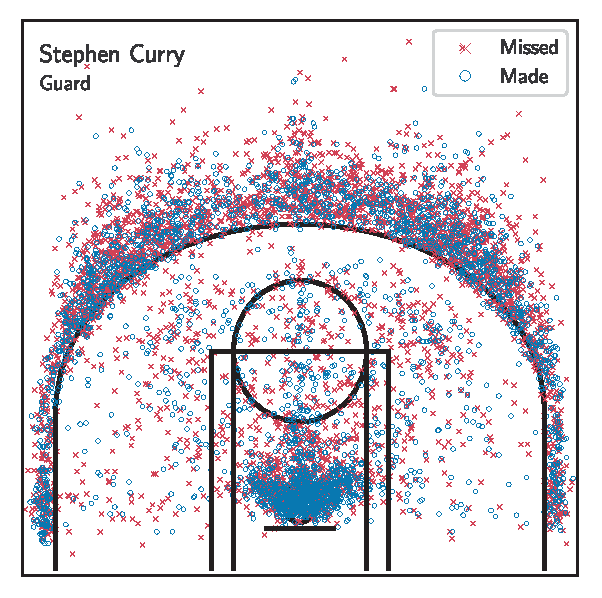
\includegraphics[scale=0.5]{figures/curry_guard.eps}
    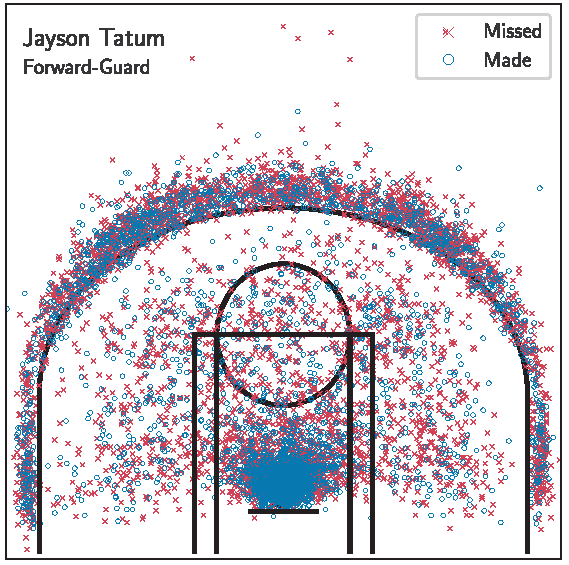
\includegraphics[scale=0.5]{figures/tatum_forward_guard.eps}
    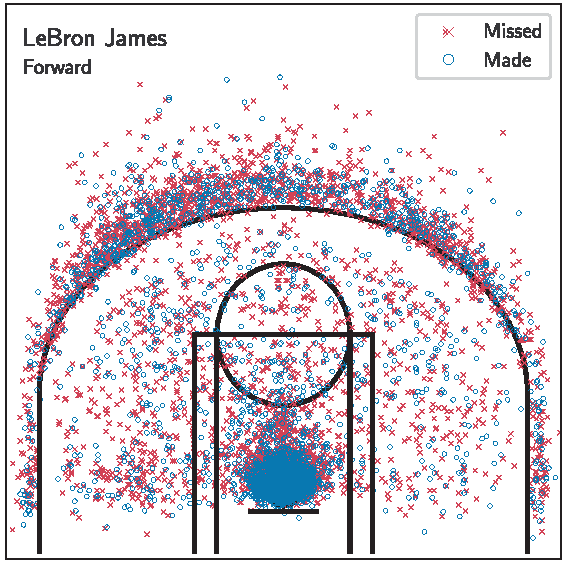
\includegraphics[scale=0.5]{figures/james_forward.eps}
    
\includegraphics[scale=0.5]{figures/embiid_forward_center.eps}
    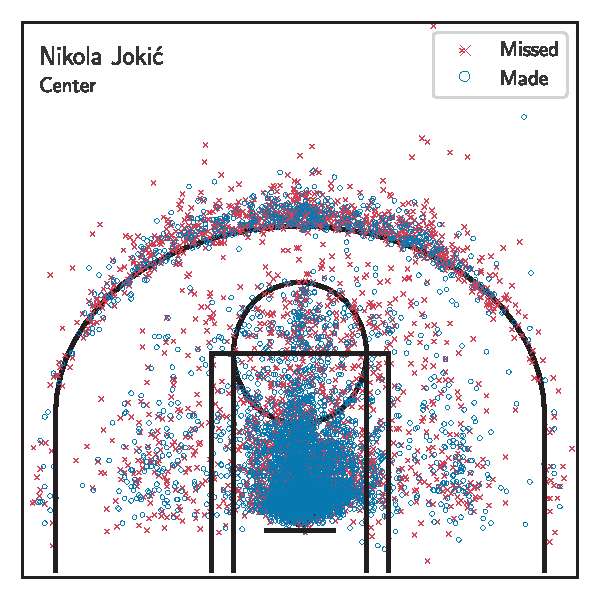
\includegraphics[scale=0.5]{figures/jokic_center.eps}
    \caption{Shots charts for five selected NBA players.}
    \label{fig:examples_shooting_charts}
\end{figure}






% section dataset (end)